\documentclass[paper=a4,fontsize=8pt,pagesize,DIV=calc]{scrartcl}
\usepackage[utf8]{inputenc}

\usepackage{fixmath,mathtools}
\usepackage{listings}
\usepackage{color}
\usepackage{array}
\usepackage{amsmath, amsfonts, amssymb}
\usepackage{multirow}
\usepackage{tabu,enumerate,tabularx}
\newcounter{row}
\usepackage{txfonts}
\usepackage{bm}
\def\Perp{\perp\!\!\!\perp}

\usepackage{here}

%% STYLE DES TABLEAUX %%
\usepackage{booktabs,tabu,longtable}
\renewcommand{\arraystretch}{1.2}

% Colonne
\usepackage{multicol}
\setlength{\columnsep}{4mm}
\setlength{\columnseprule}{1pt}

% Titre: taille
\definecolor{ao(english)}{rgb}{0.0, 0.5, 0.0}
\definecolor{applegreen}{rgb}{0.55, 0.71, 0.0}
%\usepackage{sectsty}
%\sectionfont{\color{ao(english)}\fontsize{9}{9}\selectfont}
%\subsectionfont{\fontsize{9}{9}\selectfont}
%\subsubsectionfont{\fontsize{8}{8}\selectfont}
%\paragraphfont{\color{applegreen}\fontsize{8}{8}\selectfont}

% Titre: espacements
\usepackage{titlesec}
\titlespacing\section{0pt}{-10pt plus 4pt minus 2pt}{-10pt plus 2pt minus 2pt}
\titlespacing\subsection{0pt}{-10pt plus 4pt minus 2pt}{-10pt plus 2pt minus 2pt}
\titlespacing\subsubsection{0pt}{-10pt plus 4pt minus 2pt}{-10pt plus 2pt minus 2pt}
\titlespacing\paragraph{0pt}{-13pt plus 4pt minus 2pt}{4pt plus 2pt minus 2pt}


% General document
\renewcommand{\familydefault}{\sfdefault}
\usepackage[nohead,nofoot]{geometry}
\setlength{\parindent}{0cm}
\setlength{\parskip}{4ex plus 0.3ex minus 0.1ex}
\renewcommand{\thesubsection}{\alph{subsection}.}

% Remove page number
\usepackage{nopageno}

% Itemize
\usepackage[shortlabels]{enumitem}
\setlist{nolistsep,leftmargin=*,topsep=-12pt}
\renewcommand\textbullet{\ensuremath{\bullet}}

\begin{document}

\begin{titlepage}\newgeometry{left=3cm,right=3cm,bottom=2cm,top=5cm}
\center

\newcommand{\HRule}{\rule{\linewidth}{0.5mm}}
 
%----------------------------------------------------------------------------------------
%	HEADING SECTIONS
%----------------------------------------------------------------------------------------

\textsc{\Huge Université catholique de Louvain}\\[1.5cm]
\textsc{\Huge Ecole polytechnique de Louvain}\\[0.5cm]
\textsc{\Large INMA2470: Stochastic Modelling}\\[5cm]

%----------------------------------------------------------------------------------------
%	TITLE SECTION
%----------------------------------------------------------------------------------------

\HRule \\[0.4cm]
{ \huge \bfseries FORM 2017}\\[0.4cm]
\HRule \\[1.5cm]
 
%----------------------------------------------------------------------------------------
%	AUTHOR SECTION
%----------------------------------------------------------------------------------------

\begin{minipage}{0.4\textwidth}
\begin{flushleft} \large
\emph{Author:}\\
Cynthia \textsc{Laureys}
\end{flushleft}
\end{minipage}
~
\begin{minipage}{0.4\textwidth}
\begin{flushright} \large
\emph{Professor:} \\
Philippe \textsc{Chevalier}
\end{flushright}
\end{minipage}\\[5cm]


\vfill
%----------------------------------------------------------------------------------------
%	DATE SECTION
%----------------------------------------------------------------------------------------

{\large \today}\\[3cm]

\end{titlepage}

\newgeometry{left=0.75cm, right=0.75cm, top=1.0cm, bottom=1.0cm}

\begin{center}
{\Large INMA2470 Stochastic Modelling - FORM}
\end{center}

\begin{multicols}{3}

\section{Rappels de probabilité}
\paragraph{Propriétés}
\begin{itemize}
\item Axiomes
\begin{itemize}
\item $P(\Omega)=1$ avec $\Omega=$ ensemble de réalisations
\item Pour tout évènement A, $0\leq P(A)\leq 1$
\item Si les évènements $\{A\}_i$ sont disjoints, $P(\cup_iA_i)=\sum_iP(A_i)$
\end{itemize}
\item \textbf{Loi d'addition} $P(A\cup B)=P(A)+P(B)-P(A \cap B)$
\item Proba. condit.: $P(A|B)=\frac{P(A\cap B)}{P(B)}=1-P(\bar{A}|B)$
\item Indépendance: $A/\bar{A}$ et $B/\bar{B}$ ind. $ \Leftrightarrow P(A|B)=P(A)  \Leftrightarrow P(A\cap B)=P(A)P(B)$
\end{itemize}
\paragraph{Variable aléatoire}
\begin{itemize}
\item Fonction de distribution (CFD): \\$F_X=P[X\leq x]=P[\{\omega \in \Omega:X(\omega)\leq x\}]$
\item Fonction de densité (PDF ou PMF):\\ $f_X(x)\delta \approx P[x \leq X \leq x + \delta]$
\item Espérance $\mathbb{E}[X]=$ \\ $ \sum_{x=-\infty}^{+\infty} xP[X=x]$ ou $\int^{+\infty}_{-\infty}xf(x)dx$
\begin{itemize}
\item Int. de Stieltjes: $\int^{+\infty}_{-\infty}xdF_X(x)$
\item $X\geq 0$: $\sum_{x=0}^{+\infty} (1-P(X\leq x))$ ou $\int^{+\infty}_{0}(1-F_X(x))dx$
\item $Y \equiv g(x)$: $\mathbb{E}[Y]= \int ydF_Y(y)=\int g(x)dF_X(x)$
\end{itemize}
\item Variance $\mathbb{V}(X)$=\\
$\sigma^2_X=\mathbb{E}[(X-\mathbb{E}[X])^2]=\mathbb{E}[X^2]-\mathbb{E}[X]^2$
\item m.g.f.: $g_X(r)=\mathbb{E}[exp^{rX}]$
\item $Z = X + Y$
\begin{itemize}
\item $F_Z(z) = \int_{-\infty}^{+\infty}F_X(z- y)dF_Y (y)$ (\& sym.)
\item $f_Z(z) = \int_{-\infty}^{+\infty}f_X(z- y)f_Y (y)dy $ (\& sym.)
\item $\mathbb{E}[Z]=\mathbb{E}[X]+\mathbb{E}[Y]$
\item ind: $\sigma_Z^2=\sigma_X^2+\sigma_Y^2$
\item ind: $\mathbb{E}[XY]=\mathbb{E}[X]\mathbb{E}[Y]$
\item ind: $g_Z(r)=g_X(r)\cdot g_Y(r)$
\end{itemize}
\item Comparaison $X$ et $Y$
\begin{itemize}
\item $P[X>Y]=\sum_i P[X>Y|Y=y_i]P[Y=y_i]$
\item $P[X>Y]=\int_y P[X>Y] f_Y(y) dy$
\end{itemize}
\end{itemize}
\paragraph{Loi des grands nombres}
\begin{itemize}
\item \textbf{Inégalité de Markov} pour $Y\geq 0$: $P[Y\geq y]\leq \frac{\mathbb{E}[Y]}{y}$ 
\item \textbf{Inégalité DE Chebyshev}  $P[|Z-\mathbb{E}[Z]|] \geq \epsilon]\leq \frac{\sigma_Z^2}{\epsilon^2}$
\item \textbf{Loi faible des grands nombres}:
\\ Soit $X_1$,$X_2$, ...,$X_n$ une série de variables IID ayant une espérance $\bar{X}$ et une variance $\sigma_X^2$ finies. Soit $S_n = \sum_{i=1}^n X_i$ et nous définissons la moyenne de l’échantillon $\frac{S_n}{n}$: $\lim_{n\to \infty} P\left[|\frac{S_n}{n}-\bar{X}|\geq \epsilon\right]=0$ (conv. distr.)
\item \textbf{Théorème central limite}  $\rightarrow$"$\frac{S_n}{n}\sim \mathcal{N}(\bar{X}, \frac{\sigma_X^2}{n})$"\\ $\lim_{n\to\infty} P\left[\frac{S_n-n\bar{X}}{\sqrt{n}\sigma} \leq y\right] = \int_{-\infty}^y \frac{1}{\sqrt{2\pi}} \exp\left(\frac{-x^2}{2}\right) dx$
\item \textbf{Loi forte des grands nombres} 
\\ $\lim_{n\to \infty} P\left[\sup_{m\geq n}\left(\frac{S_m}{m}-\bar{X}\right) > \epsilon\right]=0$ \\ou bien $\lim_{n\to \infty}\frac{S_n}{n}=\bar{X}$ avec prob. 1 (conv. proba.)
\end{itemize}
\section{Processus de Poisson}
Processus de renouvellement (comptage) tel que 
\\$X_i\sim_{iid} Expo(\lambda)$ \quad $S_n=\sum_{i=1}^nX_i$ \quad $\lambda=$ taux d'arrivée
\paragraph{Distribution exponentielle}
\begin{itemize}
\item $f_X(x) = \lambda \exp^{-\lambda x} $ et $F_X(x) = 1 - \exp^{-\lambda x} $ où $ x \geq 0$
\item $\mathbb{E}[X] = \frac{1}{\lambda}$
\item $\forall n, t$ $\{S_n \leq t\} = \{N(t) \geq n\}$ avec $N(t)$ processus de comptage entre $0$ et $t$
\end{itemize}
\paragraph{Propriétés}
\begin{itemize}
\item Absence de mémoire: \\ $\forall t,x>0$: $P[X>t+x|X>t]=P[X>x]$
\begin{itemize}
\item Vérifié par Expo: $P[X>t+x|X>t]=\exp^{-\lambda x}$
\item Aussi Poisson: on montre $P[Z_1>x]=\exp^{-\lambda x}$ \\ $P[Z_1>x|N(t)=0]=P[X_1>t+x|X_1>t]$ et \\ $P[Z_1>x|N(t)=n, S_n=\tau]=\frac{P[S_n=\tau, X_{n+1}>x+t-\tau]}{P[S_n=\tau,X_{n+1}>t-\tau]}$
\end{itemize}
\item $Z_m$ (temps jusqu'à $m^e$ arrivée après $t$) $\perp$ $N(t)$
\item Propriétés d'incréments stationnaires: Soit $\tilde{N} (t, t') = N(t') - N(t)$, nous avons donc que $\tilde{N} (t, t')$ à la même distribution $N(t'- t) $ $\forall t' \geq  t, t > 0$.
\item Propriété d’incréments indépendants: pour toute suite $0 < t_1 < t_2 < t_3 <... < t_k$, $\{N(t_1), \tilde{N}(t_1, t_2), \tilde{N} (t_2, t_3), ... , \tilde{N} (t_k-1, t_k)\}$ est un ensemble
de variables aléatoires indépendantes.
\end{itemize}
\paragraph{Distribution de $N(t)$}
\begin{itemize}
\item $f_{S_n}(t) = \frac{\lambda^n t^{n-1} \exp^{-\lambda t}}{(n-1)!}$ et $P[N(t) = n] = \frac{(\lambda t)^n \exp^{-\lambda t}}{n!}$
\item $\mathbb{E}[N(t)] = \lambda t$ et $\mathbb{V}[N(t)] = \lambda t$
\item Autre définition: incréments stat. et indép. +
\begin{itemize}
\item $P[ \tilde{N} (t, t + \delta) = 0] = 1 - \lambda \delta + o(\delta)$
\item $P[ \tilde{N} (t, t + \delta) = 1] = \lambda \delta + o(\delta)$
\item $P[ \tilde{N} (t, t + \delta) \geq 2] = o(\delta)$
\end{itemize}
\item Combinaison de $N_1$ et $N_2$ ind.: $N_1(t)+N_2(t)\sim Po(\lambda_1+\lambda_2)$
\item Division: Soit un processus de Poisson $N(t)$ de taux $\lambda$, les arrivées sont séparées en 2 processus $N_1$ et $N_2$, chaque arrivée étant envoyée vers le processus 1 avec une probabilité $p$
(indépendamment de l’histoire du processus).
Alors $N_1(t)\sim Po (\lambda p)$ et $N_2(t)\sim Po (\lambda (1-p))$ et sont processus sont indépendants.
\end{itemize}
\paragraph{Processus non-homogène}~~\\
Incréments indépendants mais non stationnaires avec
$\lambda(t)$ = fonction continue  à droite et $>0$.
\begin{itemize}
\item $P[N(t) = n] =\frac{(m(t))^n\exp^{-m(t)}}{n!}$ 
\item  $P[\tilde{N} (t, t') = n] =\frac{(m(t, t'))^n\exp^{-m(t,t')}}{n!}$
\item avec $m(t) = \int_0^t \lambda(\tau) d\tau$ et $m(t, t') = \int_t^{t'} \lambda(\tau) d\tau$
\end{itemize}
\paragraph{Classification de systèmes de file d'attente A/B/k}~~\\
M (exponentielle) - D (déterministe)\\
E (Erlang) - G (général)\\
Cas: \textbf{M/G/$\infty$}
\begin{itemize}
\item $N(t)$ processus de comptage des arrivées
\item $F_Y(t)$ fonction de distribution des temps de service
\item $N_1(t)$ processus de comptage des arrivées qui seront toujours en service au temps $\tau$: Poisson non-homogène de taux d'arrivée $\lambda(1 - F_Y (\tau - t))$
\item $\lim_{\tau\to \infty}m(\tau)=\lambda \mathbb{E}[Y]$
\end{itemize}
\paragraph{Symétrie et ordre}
\begin{itemize}
\item $f(s_1, s_2, ... , s_n|N(t) = n) =  \frac{
n!}{t^n}$
\item Si $\{U_1, U_2, . . . , U_n\} \sim_{iid} U(0,t)$: $g(u_1, u_2, . . . , u_n) = \frac{1}{t^n}$ $\Rightarrow $ $f_{S_1,S_2,...,S_n} =\frac{n!}{t^n}$ = var. uniformes avec ordre
\item $P[S_1 > \tau |N(t) = n]=(\frac{t-\tau}{t})^n$\\ $\Rightarrow$ $\mathbb{E}[S_1|N(t) = n] =\frac{t}{n+1}$
\item $P[X_i > \tau |N(t) = n]=P[X_1 > \tau |N(t) = n]=(\frac{t-\tau}{t})^n$\\ $\Rightarrow$ $\mathbb{E}[X_i]=(\frac{t}{n+1})$
\item $f_{S_i}(s_i|N(t) = n)=\dfrac{s_i^{i-1}(t- s_i)^{n-i} n!}{t^n(n-i)!(i-1)!}$
\end{itemize}
\section{Chaîne de Markov (nombre fini d'états)}
\paragraph{Définitions}~~\\
processus stochastique à intervalles fixes {$X_n$, $n \geq 0$} tel que chaque
variable aléatoire $X_n$, $n \geq 1$ ne dépend des variables aléatoires précédentes $X_{n-1},X_{n-2}, . . . ,X_0$ que par la
variable la plus récente \\
$P[X_n = j|X_{n-1} = i,X_{n-2} = k, . . . ,X_0 = m] $\\$= P[X_n = j|X_{n-1} = i] = P_{ij}$
\begin{itemize}
\item non-homogène si $P_{ij}(n)$
\item $j$ est accessible à partir de $i$ :\\ $i \rightarrow j \Leftrightarrow \exists n \geq 1 : P[X_n = j|X_0 = i] = P^n_{ij} > 0$ 
\\ $P^n_{ij} > 0 \Leftrightarrow$ il existe un chemin de $i$ à $j$ comprenant exactement $n$ arcs
\item $i$ et $j$ communiquent:\\
$i \leftrightarrow j$ si $i$ est accessible à partir de $j$ et $j$ est accessible à partir de $i$.
\\ $i \leftrightarrow i$ par définition
\\ si $i\leftrightarrow j$ et $m\leftrightarrow j$ alors $i \leftrightarrow m$
\item Classe d’états: ensemble d’états $T$ tel que tous les états communiquent entre eux mais les états $T$ ne communiquent avec aucun état en dehors de $T$
\item État  $i$ récurrent: $i \rightarrow j$ implique $j \rightarrow i$
\\$><$ transitoire
\\ = Propiété de classe: récurrent ou transitoire
\\ Toute chaîne de Markov avec un nombre fini d’états possède $\geq 1$ classes d’états recurrents.
\item Périodicité d’un état $i$ ($d(i)$) = PGCD des valeurs $n$ telles que $p^n_{ii} > 0$. Dit non-périodique si $d(i)=1$.
\\ = Propriété de classe
\item Si une classe récurrente a une période $d > 1$, alors $\exists$ une partition $T_1, T_2, . . . , T_d$ des états de cette classe en $d$
sous-ensembles telle que toutes les transitions à partir d’un état du sous-ensemble $T_n$ vont vers un état de $T_{n+1}$ et toutes les transitions à partir d’un état de $T_d$ vont vers un état de $T_1$.
\\ Si $j\in T_n$ et $p_{jk} > 0$ alors $k \in T_n+1$.
\item Classe ergodique = non périodique + récurrente
\end{itemize}

\paragraph{Equation de Chapman-Kolmogorov}~~\\
$P^2_{ij}=\sum_{k=1}^J P_{ik}P_{kj}$\\$\Rightarrow$ $P^2=P.P$ et $ P^n=P.P.P...P $ (n times)
\\ Général: $P^{m+n}_{ij} =\sum^J_{k=1}P^m_{ik} P^n_{kj}$ et $P^{m+n} = P^m.P^ n$
\paragraph{Convergence}
\begin{itemize}
\item $P$ est une matrice stochastique \\$\Leftrightarrow$ carrée, non-négative et somme de chaque ligne $=1$ ($Pe=e$)
\item "unichain"= chaîne de Markov qui contient au plus une classe récurrente (+états transitoires)
\item $\pi=$ vecteur des probabilités stationnaires tel que:
$\pi=\pi P$ où $\sum_i \pi_i=1;\pi_i\geq 0,1\leq i \leq M$
\\  = vecteur propre à gauche, autant de solutions que de classes récurrentes (multiplicité de la valeur propre 1). Si $>1$, alors $P^{\infty}$ a des lignes $\neq $
\item Unicité de $\pi$ si "unichain": toutes les rangées convergent vers le vecteur ligne $\pi$:\\ $\lim_{n\to \infty}P^n=e\pi$
 alors $P^{\infty}=P^{\infty}P \Rightarrow \pi = \pi P$
\item Convergence de $P^n$ si pas de classe périodique  $\rightarrow $ sinon $\pi$  pris comme moyenne sur sous-classes
\end{itemize}
\paragraph{Chaîne de Markov avec gains en régime transitoire}
\begin{itemize}
\item $r_{ij}=$ gain associé à la transition $i$ vers $j$
\item $r_i=\sum_j P_{ij}r_{ij} =$ espérance du gain à l'état $i$
\item $g=\sum_i r_i\pi_i =\pi \bm{r}$ gain moyen par période
\item Pour un horizon de longueur $n$:\\ étapes $n\rightarrow 0$ et périodes $0\rightarrow n$
\item Gain pour l'étape $n$: $v_i(n)=r_i+\sum_j P_{ij}v_j (n-1)$
\\$\bm{v}(n)=\bm{r}+\bm{P}\bm{v}(n-1)$
\\ $\bm{v}(n)=\bm{r}+\bm{Pr}+\bm{P}^2\bm{r}+...+\bm{P}^{n-1}\bm{r}+\bm{P}^n\bm{v}(0)$
\end{itemize}
\paragraph{Convergence}~~\\
Supposons $\bm{v}(n)\approx \bm{w}+ng \bm{e}+\beta \bm{e}$ avec $w_i$ l'avantage relatif de démarrer de l'état $i$ et $\beta$ une constante
\begin{itemize}
\item \textbf{Lemme 1} Soit $\bm{P}$ une matrice de transition d’une chaîne de Markov ayant une seule classe récurrente, alors le système $\bm{w} + g\bm{e} = \bm{r} + \bm{Pw}$ admet toujours une solution $w$, en ajoutant la condition $w_1 = 0$ (ou autre), la solution est unique.
\item \textbf{Théorème 1} Soit $\bm{P}$ une matrice de transition d’une chaîne de Markov ayant une seule classe récurrente, alors 
$\lim_{n\rightarrow \infty}(\bm{v}(n) - ng\bm{e}) = \bm{w} + \beta\bm{e}$ avec $\beta =\sum_i \pi_i (v_i(0) - w_i)$
\\ $\bm{v}(n)-ng\bm{e}=\bm{w}+\bm{P}^n(\bm{v}(0)-\bm{w})$
\end{itemize}
\paragraph{Processus de décision markovien}~~\\
Pour chaque état $i$, choix entre $K_i$ possibilités avec des gains $r_i^{(1)},r_i^{(2)},...,r_i^{(K_i)}$ et des probas de transitions correspondantes:\\ $\{P_{ij}^{(1)},1\leq j\leq J\},P_{ij}^{(2)},1\leq j\leq J\},...,P_{ij}^{(K_i)},1\leq j\leq J\}$
\begin{itemize}
\item Politique dynamique optimale $B$ si
\\$\bm{r}^B + \bm{P}^B\bm{v}^*(n - 1)\geq \bm{r}^A + \bm{P}^A\bm{v}^*(n - 1) \quad \forall A$
\begin{itemize}
\item $v^*_i (n) = max_k\{r^{(k)}_i +\sum_j P^{(k)}_{ij} v^*_j (n - 1)\}$
\item $\bm{v}^*(n) = max_A\{\bm{r}^A + \bm{P}^A\bm{v}^*(n - 1)\}$
\end{itemize}
\item Hypothèse: Pour toute politique $A$ la chaîne de Markov avec matrice de transition $\bm{P}^A$ possède une seule classe
récurrente.
\item Politique stationnaire optimale $B$ si maximise $g^B$
\begin{itemize}
	\item $\bm{v}^A(n)-ng^A\bm{e}=\bm{w}^A+[\bm{P}^A]^n(\bm{v}(0)-\bm{w}^A)$
	\item $\bm{w}^A + g^A\bm{e} = \bm{r}^A + \bm{P}^A\bm{w}^A$
	\item Pour les étapes $n>m$, la politique dyn. opti.= stat. opti.
	\item Si $B$ stationnaire optimale, $B$ ergodique, pour $n>>m,$ $v_i^*\approx w_i^B+c(n)$
\item $B$ dyn. opti. si $\bm{r}^B+\bm{P}^B\bm{w}^B\geq \bm{r}^A+\bm{P}^A\bm{w}^A$ $\forall A$	
	\end{itemize}
\item \textbf{Lemme 2} Si $\bm{v}(0) = \bm{w}^B$ pour une politique B et si $\bm{r}^B + \bm{P}^B\bm{w}^B \geq  \bm{r}^A + \bm{P}^A\bm{w}^B +A$ alors $B$ est la politique dynamique optimale pour toutes les étapes et $\bm{v}^*(n) = \bm{w}^B + ng^B\bm{e}$
\item \textbf{Théorème 2} Si pour toute politique $A$ la chaîne de Markov $P^A$ est récurrente alors la politique $B$ est une politique stationnaire optimale ssi 
\\$\bm{r}^B + \bm{P}^B\bm{w}^B \geq \bm{r}^A + \bm{P}^A\bm{w}^B \quad \forall A$
\item \textbf{Algorithme} d’amélioration successives (Howard)
\begin{enumerate}
\item Choisir une politique arbitraire $B$
\item Calculer $\bm{w}^B$
\item Si $\bm{r}^B + \bm{P}^B\bm{w}^B \geq \bm{r}^A + \bm{P}^A \bm{w}^B  \quad \forall A $  stop
\\Sinon continuer
\item  Trouver $A$ tel que $\bm{r}^A + \bm{P}^A\bm{w}^B \geq \bm{r}^B + \bm{P}^B\bm{w}^B$
\\ Choix de $A$? On choisit souvent $k_i=\arg \max_k r_i^{(k)}+\sum_j P_{ij}^{(k)}w_j^B$
\item $B \rightarrow A$ retour en 2
\end{enumerate}
\item \textbf{Lemme 3} Soit $\bm{v}(0)$ et $\bm{v}'(0)$ deux vecteurs de gain final tels que $\bm{v}(0) \leq v'(0)$. Alors pour toute politique stationnaire $A$, $\bm{v}^A(n) \leq \bm{v}'^A(n) \forall n$, pour la politique dynamique optimale $\bm{v}^*(n) \leq  \bm{v}'^*(n) \forall n$
\\ Soit $B$ une politique stationnaire optimale et $\gamma$ tel que $\bm{v}(0) \leq  \bm{w}^B + \gamma \bm{e}$, nous aurons dès lors $\bm{v}^*(n) \leq  (ng^B + \gamma)\bm{e} + \bm{w}^B$
\item \textbf{Lemme 4} Soit $B$ une politique stationnaire optimale alors $f(n) = \bm{\pi}^B\bm{v}^*(n) - ng^B$ est monotone et croissante en $n$, et $\lim_{n\to \infty } f(n) = \beta'$
\item \textbf{Théorème 3} Supposons que $\bm{P}^A$ est récurrente pour tout $A$, que $B$ est une politique stationnaire optimale avec $\bm{P}^B$ ergodique alors
\\ $\lim_{n\to \infty} \bm{v}^*(n) - ng^B \bm{e} = \bm{w}^B + (\beta'- \bm{\pi}-\bm{\pi}^B\bm{w}^B)\bm{e}$
\begin{itemize}
\item Gain moyen de la politique dynamique optimale $= g^B$
\item Gain relatif de la politique dynamique optimale $= \bm{w}^B$
\item Gain relatif de toutes les politiques stationnaires optimales sont identiques !
\item $\min_i[v_i^*(n) - v^*_i (n - 1)] \leq g^B \leq \max_i[v^*_i(n) - v^*_i (n - 1)]$
\end{itemize}
\item \textbf{Algorithme de programmation dynamique}
\begin{enumerate}
\item Fixer arbitrairement $\bm{v}(0)$
\item Calculer $\bm{v}^*(n) = \max_A{\bm{r}^A + \bm{P}^A\bm{v}^*(n - 1)}$
\item Calculer $l = \min_i [v^*_i (n) - v^*_i (n - 1)]$ et $ u = \max_i[v^*_i (n) - v^*_i (n - 1)]$
\item Tant que $l < u$ recommencer à l’étape 2
\item $ A$ est la politique stationnaire optimale et le gain stationnaire maximum est $l = u = g^A$.
\end{enumerate}
\end{itemize}
\section{Processus de renouvellement}
$\{N(S_n + t) - N(S_n); t \geq 0\}$ est un processus stochastique qui a la même distribution que $N(t)$.
\paragraph{Notations}
\begin{itemize}
\item $X_i$ temps entre arrivées (renouvellements)
\item $\bar{X}= \mathbb{E}[X]$ supposé fini avec $P[X_i >0] =1$
\item $\sigma$ peut être infini
\item $S_n =\sum_{i=1}^n X_i$
\end{itemize}
\paragraph{Propriétés}
\begin{itemize}
\item \textbf{Lemme 1} Soit $\{N(t); t \geq 0\}$ un processus de renouvellement. Alors
$\lim_{t\to\infty}N(t) = \infty$ avec prob. 1
et $\lim_{t\to\infty}\mathbb{E}[N(t)] = \infty$.
\item \textbf{Théorème 1} $\lim_{t\to\infty}
\frac{N(t)}{t}=\frac{1}{\bar{X}}$ avec prob. 1
\item \textbf{Théorème central limite} ($\sigma<\infty$):
\\$\lim_{t\to\infty}P\left[ \frac{N(t)-t/\bar{X}}{\sigma \bar{X}^{-3/2}\sqrt{t}}<\alpha\right]=\Phi(\alpha)$
\\$\Rightarrow P\left[ S_n\leq n\bar{X}+\alpha \sqrt{n}\sigma \right]\approx \Phi(\alpha)$
\\ assympt. exact avec $t=n\bar{X}+\alpha \sqrt{n}\sigma$
\end{itemize}
\paragraph{Règle d'arrêt}~~\\
$N$ v.a. = nbr total d’expériences observées
\begin{itemize}
\item \textbf{Règle de décision} $\{I_n; n \geq 1\}$ tel que 
\\$I_n = \begin{cases} 1 & \text{ si $n^e$ expérience est observée}\\0 &\text{ sinon} \end{cases}$
\\$I_n$ = fonction indicatrice de $\{N \geq n\}$.
\item \textbf{Règle d’arrêt} pour une série de v.a. $\{X_n; n \geq 1\}$ est une v.a. entière positive $N$ telle que $\forall n$
\begin{itemize}
\item la fonction indicatrice $  I_n$ de $\{N \geq n\}$ est une fonction de $X_1, ... ,X_{n-1}$, avec $I_1 = 1$.
\item $\{I_n|X_1, ...,X_{n-1}\}$ est indép. de $\{X_i; i \geq  n\}$.
\end{itemize}
\item \textbf{Égalité de Wald} Soit $N$ une règle d’arrêt pour $\{X_n; n \geq 1\}$ alors
$\mathbb{E}[S_N] = \bar{X} \mathbb{E}[N]$
\item \textbf{Théorème élémentaire de renouvellement} $\lim_{t\to\infty}\frac{\mathbb{E}[N(t)]}{t}=\frac{1}{\bar{X}}$
\item Distribution arithmétique: processus de renouvellement a une distribution arithmétique ssi les arrivées ne peuvent se produire que pour des moments qui sont des multiples d’un nombre réel $d > 0$. (pas de la distribution)
\item \textbf{Théorème de Blackwell} Si la distribution des temps entre renouvellement est
\begin{itemize}
\item  non-arithmétique
\\$\lim_{t\to\infty}[m(t + \delta) - m(t)] =
\frac{\delta}{\mathbb{E}[X]} \forall \delta$
\item arithmétique de pas $d$
\\$\lim_{t\to\infty}[m(t + nd) - m(t)] =
\frac{nd}{\mathbb{E}[X]} \forall n\geq 1$
\end{itemize}
\item Lien avec proc de Poisson: 
\\pour distr non-arithmétique avec $P[X_i = 0] = 0$
\begin{itemize}
\item $\lim_{t\to\infty} P[N(t + \delta) - N(t) = 0] = 1 - \frac{\delta}{\bar{X}} + o(\delta)$
\item $\lim_{t\to\infty}P[N(t + \delta) )- N(t) = 1] = \frac{\delta}{\bar{X}} + o(\delta)$
\item $\lim_{t\to\infty}P[N(t + \delta) - N(t) \geq 2] = o(\delta)$
\end{itemize}
\item  assympt. incréments stationnaires mais pas indép.
\item  La somme d'un grand nombre de processus indépendants aura des incréments très proches d'être indépendants
\end{itemize}
\section{Renewal reward process}
\paragraph{Reward function} $R(t)$ 
\begin{itemize}
\item random variable: rate at which the process is accumulating a reward/cost
\item can only depend on the
current renewal
\end{itemize}
Examples
\begin{itemize}
\item $R(t) = Y (t) = S_{N(t)+1} -t$
\\=Residual life at time $t$ for the current renewal
\\Time average:  $\lim_{t\to\infty} \frac{1}{t} \int_0^t Y(\tau) d\tau=\frac{\mathbb{E}[X^2]}{2\mathbb{E}[X]}=\frac{1}{2}\mathbb{E}[X]+\frac{1}{2}\frac{\mathbb{V}[X]}{\mathbb{E}[X]}>\frac{1}{2}\mathbb{E}[X]$ avec prob. 1
\item$R(t) = Z(t) = t - S_{N(t)}$
\\=Age at time $t$ of the current renewal
\\Time average:  $\lim_{t\to\infty} \frac{1}{t} \int_0^t Z(\tau) d\tau=\frac{\mathbb{E}[X^2]}{2\mathbb{E}[X]}$
\item$R(t) = X(t) = S_{N(t)+1}- S_{N(t)}$
\\=Duration of the renewal containing time $t$
\\Time average:  $\lim_{t\to\infty} \frac{1}{t} \int_0^t X(\tau) d\tau=\frac{\mathbb{E}[X^2]}{\mathbb{E}[X]}$
\end{itemize}
\paragraph{Accumulated reward} during the $n^{th}$ renewal: $R_n$ 
\begin{itemize}
\item $R_n =\int^{S_n}_{S_{n-1}} R(\tau )d\tau =\int^{S_n}_{S_{n-1}} R(Z(\tau ), X(\tau ))d\tau$\\$=\int^{S_n}_{S_{n-1}} R(\tau-S_{n-1},X_n)d\tau = \int^{X_n}_0 R(z, X_n)dz$
\item IID r. v. (like $X_n$): depends on $X_n$ and $R(z,x)$
\item $\mathbb{E}[R_n] =\int_{x=0}^{\infty}R_ndF_X(x)=\int_{x=0}^{\infty}\int_{z=0}^xR(z,x)dz df_X(x)$
\item \textbf{Théorème} Let $R(t)$ be a renewal reward function for a renewal process with expected inter-renewal times $\bar{X}<\infty$, then with prob.1: $\lim_{t\to\infty} \frac{1}{t}\int_0^t R(\tau)d\tau=\frac{\mathbb{E}[R_n]}{\bar{X}}$
\end{itemize}
\paragraph{Distribution of residual life}~~\\
$R(t)=I\{Y(t)\leq y\} \quad R_n=\min\{y,X_n\}$
\begin{itemize}
\item $\mathbb{E}[R_n] = \mathbb{E}[\min \{y,X_n\}]$\\$=\int_0^\infty P[\min\{ y,X_n\} >x]dx=\int_0^y P[X>x]dx$
\item $F_Y (y) =\lim_{t\to\infty} \frac{1}{t}\int_0^t R(\tau )d\tau =\frac{\mathbb{E}[R_n]}{\bar{X}}$\\$=\frac{1}{\bar{X}}\int_0^y  P[X>x]dx$
\end{itemize}
\paragraph{Ensemble average}
Suppose $t$ sufficiently large such that $m(\tau+\delta) - m(\tau ) =\frac{\delta }{\bar{X}}$ for
all $\tau$ close to $t$.
\\$P[Z(t)\in (z, z + \delta), X(t) \in (x, x + \delta)]$
\\$= P[$ renewal $ \in (t- z-\delta, t-z),$  interval $\in(x, x + \delta)]$
\\$=\frac{\delta}{\bar{X}}\delta f_X(x)+ o(\delta^2) = \frac{\delta^2f_X (x)}{\bar{X}}+ o(\delta^2)$
\\$\Rightarrow f_{Z(t),X(t)}(z, x) =\begin{cases} \frac{f_X (x)}{\bar{X}}& \text{ if } x > z\\ 0 & \text{ otherwise }\end{cases}$
\paragraph{Key Renewal theorem}~~\\
Let $N(t)$ be a non-arithmetic renewal process, let $R(z, x) \geq 0$ be such that $r (z) =\int_{x=z}^\infty R(z,x)dF_X (x)$ is directly Rieman integrable. 
\\ Then $\lim_{t\to\infty} \mathbb{E}[R(t)]=\frac{\mathbb{E}[R_n]}{\bar{X}}$
\paragraph{Application: Little's Law}~~\\
General queueing system:
\begin{itemize}
\item $A(t)$ the number of arrivals between $0$ and $t$
\item $D(t)$ the number of departures between $0$ and $t$
\item $L(t) = A(t) - D(t)$ the number of customers in the system at time $t$
\item $L_q(t)$ number of customers in queue at time $t$
\item $w_i$ the time the $i^{th}$ customer spends in the system
\item $N(t)$ renewal process counting the number of busy periods of the system (each time a customer arrives when system is empty)
\end{itemize}
$\Rightarrow L(t)$ reward function for the renewal process $N(t)$
Little's Law ($\lambda=$arrival rate, $\bar{Z}=$ expect. service time)
\begin{itemize}
\item Av. customers in system: $\bar{L}=\lambda \bar{W}$
\item Av. customers in the queue: $\bar{L}_q=\lambda \bar{W}_q$
\item Av. customers being served: $\rho=\lambda \bar{Z}$ 
\end{itemize}
Cas: \textbf{ M/G/1}
\begin{itemize}
\item $R(t)$ remaining time for the customer being served ($=0$ if server is idle)
\item $U(t)$ time an arrival at time $t$ would have to wait before being served (workload in the system): $U(t) =\sum_{i=1}^{L_q(t)} Z_i +R(t)$
\\$\mathbb{E}[U(t)] = \mathbb{E}[L_q(t)]\mathbb{E}[Z] + \mathbb{E}[R(t)]$ \\(as $L_q(t)$ and $Z_i$ ind.)
\\$\lim_{t\to\infty}\mathbb{E}[U(t)]=\lambda \bar{W}_q\mathbb{E}[Z]+\lambda\frac{\mathbb{E}[Z^2]}{2}$
\item $\mathbb{E}[W_q(t)]=\mathbb{E}[U(t)]$ (arrivées selon Poisson)
\\$\Rightarrow \bar{W}_q= \frac{\lambda \mathbb{E}[Z^2]}{2(1 -\lambda\mathbb{E}[Z])}$
\item $\bar{W}=\bar{W}_q+\mathbb{E}[Z]$
\end{itemize}
\section{Chaîne de Markov (nombre infini d'états)}
\paragraph{Définitions/Propriétés}
\begin{itemize}
\item $f_{ij}(n)$: proba. de $1^{er}$ passage  en $j$ pour $X_0=i$
$f_{ij}(n) = P[X_n = j,X_{n-1} \neq j, ... ,X_1\neq j|X_0 = i]$
\\$f_{ij}(n) =\sum_{k\neq j} p_{ik}f_{kj}(n - 1)$
\\ $f_{ij}(1) = p_{ij}$
\item $F_{ij}$: proba. au plus tard en $j$ pour $X_0=i$
\\$F_{ij}(n)=\sum_{m=1}^{n}f_{ij}(m)$
\item $T_{ij}$ v.a.: temps jusqu'au premier passage en $j$ 
\\$\bar{T}_{ij}=1+\sum_{n=1}^\infty (1-F_{ij}(n))$
\item État récurrent ($F_{ij}(\infty)=1$) \\ou transitoire ($F_{ij}(\infty)<1$) 
\begin{itemize}
\item nul-récurrent: $\bar{T}_{jj} =\infty$
\item positif récurrent: $\bar{T}_{jj}<\infty$
\end{itemize}
\item \textbf{Théorème 1} Tous les états d’une même classe sont du même type (transitoire, nul-récurrent, positif-récurrent).
\item \textbf{Théorème 2} Soit $j$ un état récurrent non-périodique et $i$ un état dans la même classe que $j$ alors
$\lim_{n\to\infty}P[X_n = j|X_0 = i] =\frac{1}{\bar{T}_{jj}}$
\item Chaîne de Markov irréductible: si
tous les états communiquent entre eux.
\item \textbf{Théorème 3} Soit une chaîne de Markov irréductible, si le système
$\begin{cases}\pi_j=\sum_i \pi_i p_{ij} \forall j\\ \sum_j \pi_j=1\\ \pi_j\geq 0 \forall j\end{cases}$
possède une solution, alors $\pi_i = 1/\bar{T}_{ii}$ et tous les états sont positif-récurrent.
\\ Si les états sont positifs-récurrents alors le système possède une solution.
\end{itemize}
\paragraph{Chaînes de naissance et de mort}~~\\
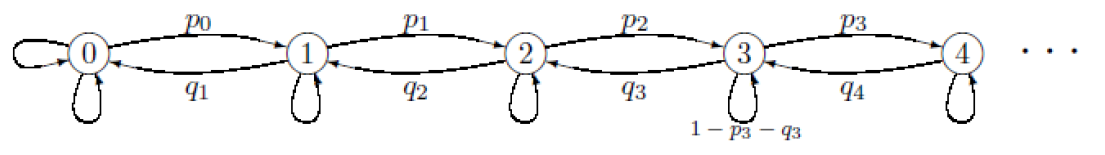
\includegraphics[width=0.3\textwidth]{Death}
$\pi_ip_i = \pi_{i+1}q_{i+1}.$ \quad $\rho_i=\frac{p_i}{q_{i+1}} \quad \Rightarrow \pi_{i+1}=\rho_i\pi_i$
\\$\Rightarrow \pi_i=\pi_0 \prod_{j=0}^{i-1} \rho_j$ \quad $\Rightarrow \pi_0=\frac{1}{1+\sum_{i=1}^\infty \prod_{j=0}^{i-1} \rho_j}$
\\ Si $\rho_i =\rho \  \forall i \Rightarrow \rho<1 \Rightarrow$ convergence, les états sont tous positif-récurrents.
\begin{itemize}
\item Homogénité (Markov):$[E^+|X_n,E^-]=P[E^+|X_n]$ et $[E^-|X_n,E^+]=P[E^-|X_n]$
\item Si la chaîne est dans l’état stationnaire alors la chaîne inverse est homogène.
\\ $P[X_{n-1} = j|X_n = i] = P[X_n = i|X_{n-1} = j]\frac{\pi_j}{\pi_i}$
\\$p^*_{ij}=p_{ij}\frac{\pi_j}{\pi_i}$
\item Une chaîne est réversible si $p^*_{ij}=p_{ij} \ \forall i,j$
\\ C'est-à-dire $\pi_ip_{ij}=\pi_j p_{ji}$
\item \textbf{Théorème 4}  Toute chaîne de naissance et de mort qui possède une distribution stationnaire est réversible.
\item \textbf{Théorème 5} Soit une chaîne de Markov irréductible avec des probabilités de transition $p_{ij}$. Soit une série de nombres positifs $\{\pi_i\}$ tels que $\sum_i \pi_i=1$ et tels que $\pi_ip_{ij} = \pi_jp_{ji} \ \forall i j$ alors $\{\pi_i\}$ sont les probabilités stationnaires de la chaîne de Markov et la chaîne est réversible.
\item \textbf{Théorème 6} Soit une chaîne de Markov irréductible avec des probabilités de transition $p_{ij}$. Soit une série de nombres positifs $\{\pi_i\}$ tels que $\sum_i \pi_i=1$. Soit $P^*$ une matrice de probabilités de transition telle que
$\pi_ip_{ij} = \pi_jp^*_{ji}$ $\forall i,j$  alors $\{\pi_i\}$ sont les probabilités stationnaires de la chaîne de Markov et $P^*$ est la matrice de transition de la chaîne inverse.
\end{itemize}
\paragraph{Exemple: Systèmes à temps partagé}~~\\
Système “round-robin” : chaque demande à son tour est traitée durant un petit temps $\delta$ (quand $\delta\rightarrow 0$ on a
un système à temps partagé).
\\Supposons un incrément $\delta$ et $W$ temps de service est arithmétique avec pas $\delta$. 
\\Soit $f(j) = P[W = j\delta]$, $ \bar{F}(j) = P[W > j\delta ]$
\\$P$[client déjà servi durant $j$ périodes termine en $j + 1$] $=\frac{f(j+1)}{\bar{F}(j)} = g(j)$
\\État du système : $s = (m, z_1, z_2, ... , z_m)$
\\ Si il n’y a personne $s = (0) = \varnothing$
\\Transitions possibles pour $X_n \neq \varnothing$ dans l’ordre :
\begin{enumerate}
\item une arrivée dans le système avec proba $\lambda\delta$ (tjs en $1^e$ position)
\item le client en première position est servi durant $\delta$
\item le client part si son service est terminé
\item le client va en fin de file
\end{enumerate}
\begin{itemize}
\item Si pas d’arrivée, pas de départ $\Rightarrow $ rotation: $s \rightarrow r(s) = (m, z_2, z_3, ... , z_m, z_1 + 1)$
\item Si départ $s \rightarrow d(s) = (m - 1, z_2, z_3, . . . , z_m)$
\item Si arrivée $s\rightarrow a(s) = (m + 1, z_1, z_2, z_3, ... , z_m, 1)$
\end{itemize}
Probabilités de transition
\\$p_{s,r(s)} = (1 - \lambda\delta)(1 - g(z_1))$ \qquad 
$p_{s,d(s)} = (1 -\lambda\delta)g(z_1)$
\\$p_{s,a(s)} = \lambda\delta(1 -f(1))$ \qquad
$p_{s,s} = \lambda\delta f(1)$
\\$p_{\varnothing\varnothing} = (1-\lambda\delta) + \lambda\delta f(1)$ \qquad
$p_{\varnothing(1,1)} = \lambda\delta(1 - f(1))$
\paragraph{Exemple: Systèmes à temps partagé(Inverse)}~~\\
Un round-robin aussi où l’état $s = (m, z_1, z_2, . . . , z_m)$ indique le nombre de périodes restant afin que chaque client termine son service.
La rotation se fait dans le sens inverse, et le premier client sur lequel on travaille est $z_m$. Les arrivées se font suivant un processus de Bernouilli de paramètre $\lambda\delta$.
\\$p^*_{r(s),s} = (1-\lambda\delta)$ \qquad $p^*_{a(s),s} = (1 -\lambda\delta)$ 
\\ $p^*_{d(s),s} =\lambda\delta f(z_1 + 1)$ \qquad $p^*_{s,s} = \lambda\delta f(1)$
\\À vérifier: $\pi_ip_{ij}=\pi_j p^*_{ji}$
\\D'où $\pi_s = \frac{ \lambda\delta }{1- \lambda\delta }\bar{F}(z_1)\pi_{d(s)} =\left(\frac{ \lambda\delta }{1- \lambda\delta }\right)^2 \bar{F}(z_1)\bar{F}(z_2)\pi_{d(d(s))}$ $\Rightarrow \pi_s =\left(\frac{ \lambda\delta }{1- \lambda\delta }\right)^m \prod_{j=1}^m \bar{F}(z_j)\pi_{\varnothing}$
\\Notez : $1 - g(z_1) =\frac{\bar{F}(z_1-f(z_1+1)}{\bar{F}(z_1)} =\frac{\bar{F}(z_1+1)}{\bar{F}(z_1)}$
\\ D'où $(1 -\lambda\delta) \frac{\bar{F}(z_1+1)}{\bar{F}(z_1)} \left(\frac{\lambda\delta}{1-\lambda\delta}\right)^m \prod_{j=1}^m \bar{F}(z_j)\pi_\varnothing \\=(1 -\lambda\delta)  \left(\frac{\lambda\delta}{1-\lambda\delta}\right)^m \prod_{j=2}^m \bar{F}(z_j)\bar{F}(z_1+1)\pi_\varnothing $
\\Soit la probabilité d’avoir $m$ clients :
\\$p_m =\sum_{z_1,...,z_m}\pi(m,z_1,...,z_m) $\\$=\left(\frac{\lambda\delta}{1-\lambda\delta}\right)^m \prod_{j=1}^m\left(\sum_{i=1}^{\infty}\bar{F}(si)\right)\pi_\varnothing$
\\ $\delta \sum_{i=1}^\infty \bar{F}(z_i)=\mathbb{E}[W]-\delta$
\\ $p_m=\left(\frac{\lambda}{1-\lambda\delta}\right)^m(\mathbb{E}[W]-\delta)^m \pi_\varnothing$
\\$\rho=\left(\frac{\lambda}{1-\lambda\delta} \right)(\mathbb{E}[W]-\delta),$ $p_m=\rho^m\pi_\varnothing$ $\Rightarrow \pi_\varnothing=1-\rho$
\\Nombre moyen de clients $L =\sum_{m=1}^{\infty}mp_m=\frac{\rho}{1-\rho}$
\\Little $\Rightarrow$ attente moyenne $W =\frac{\rho}{\lambda(1-\rho)}$
\\ Notez que $L$ et $W$ ne dépend pas de $\sigma$
\section{Processus semi-Markovien}
\paragraph{Définition}= une chaîne de Markov où les intervalles entre transitions sont des variables aléatoires. 
\\Soit $S_1 < S_2 < S_3 < ...$ les temps des transitions successives.
\\Soit $U_n = S_n -S_{n-1}$ (dépend que de $X_{n-1}$ et $X_n$)
\\Soit les états successifs $X_0,...,X_n$,
\\ $X(t) = X_n$ $\forall t \in S_n \leq  t < S_{n+1}$.
\\$P[U_n\leq  u|X_{n-1} = i,X_n = j] = G_{ij}(u)$
\\ $\mathbb{E}[U_n|X_{n-1} = i,X_n = j] = \bar{U} (i, j)$
\paragraph{Probabilités stationnaires}
\begin{itemize}
\item \textbf{Théorème 1} Si la chaîne sous-jacente est irréductible et récurrente positive alors les probabilités stationnaire d’être dans l’état $i$, $p_i$ est donnée par :
$p_i =\frac{\pi_i \bar{U}(i)}{\sum_j \pi_j\bar{U} (i)}$
\\ Où $\bar{U} (i) = \mathbb{E}[U_n|X_{n-1} = i] = \sum_j P_{ij}\bar{U} (i, j)$
\item Soit $M(t)$ le nombre de transitions jusque $t$. On peut montrer que $\lim_{t\to\infty}M(t) = \infty $ avec prob. 1.
\item Soit $M_{ij}(t)$ le nombre de transitions vers l'état $j$ jusqu'au
temps $t$ étant donné que $X_0 = i$.
$M_{ij}(t)$ est un processus de renouvellement avec délai.
Considérons un gain $R(t)$ de $1$ tant que $X(t) = j$ et $0$ sinon.
\\$p_j = \lim_{t\to\infty}\frac{\int_0^t R(\tau)d\tau}{t}=\frac{\bar{U}(j)}{\bar{W}(j)}$
\\où $\bar{W}(j)=$ l’espérance du temps entre deux passages par l’état $j$.
\item Par la loi des grands nombres : \\$\lim_{t\to\infty}\frac{M_{ij}(t)}{t}=
\frac{1}{\bar{W}(j)}$.
\\ Soit $N_{ij}(n)$ le nombre de passages par l’état $j$ dans les $n$ premières transitions.
\\On a $M_{ij}(t) = N_{ij}(M(t))$ et $\lim_{t \to \infty}\frac{M_{ij}(t)}{M(t)}=\lim_{t\to\infty}\frac{N_{ij}(M(t))}{M(t)}=\lim_{n\to\infty}\frac{N_{ij}(n)}{n}=\pi_j$
\\ $p_j=\bar{U}(j)\pi_j \lim_{t\to\infty}\frac{M(t)}{t}$
\\$\lim_{t\to\infty} \frac{M(t)}{t}=\frac{1}{\sum_j \pi_j \bar{U}(j)}$
\item$ Q(i, j)=$  probabilité que le processus soit en transition
entre l’état $i$ et $j$: $Q(i, j) = p_i \frac{p_{ij}\bar{U}(i, j)}{\bar{U}(i)}$
\end{itemize}
\section{Processus de Markov}
\paragraph{Définition} = processus semi-markovien avec des distributions exponentielles pour les transitions.
La distribution ne dépend que de l'état de départ et $p_{ii} = 0$. $P[U_n\leq  x|X_{n-1} = i,X_n = j] = 1 -\exp^{-\nu_ix}$
\begin{itemize}
\item irréductible si la chaîne de Markov sous-jacente est irréductible
\item $Y (t)$ le temps résiduel jusqu’à la prochaine transition:
\\ $P[Y (t)\leq x,X(t+Y (t)) = j|X(t) = i, \{X(\tau );\tau < t\}] = p_{ij}(1-\exp^{-\nu_ix})$
\item Si $x$ tout petit:
$P[X(t + \delta) = j|X(t) = i, \{X(\tau <t\}] = \nu_i p_{ij}+o(\delta)$
\\$\Rightarrow$ Taux de transition$= q_{ij} = \nu_i p_{ij}$ avec
 $\nu_i= \sum_j q_{ij}$
 \item $P[Y (t)= x,X(t+Y (t)) = j|X(t) = i, \{X(\tau );\tau < t\}] =P[Y (t)= x,X(t+Y (t)) = j|X(t) = i] $ (Pas mémoire)
 \item 3 manières
 \begin{enumerate}
 \item Processus semi-markovien avec transition $expo(\nu_i)$ et choix état suivant $j$ avec probabilité $p_{ij}$
 \item $N$ processus de $Poisson(\nu_i)$, si $X(t) = i$ alors transition quand prochaine arrivée du processus $i$ et choix état
suivant $j$ avec probabilité $p_{ij}$
\item $N^2$ processus de $Poisson(q_{ij})$ si $X(t) = i$ alors transition quand arrivée du premier processus $ij$ et transition vers
l’état $j$ correspondant à cette première arrivée Processus.
 \end{enumerate}
 \end{itemize}
 \paragraph{Probabilités stationnaires}
 \begin{itemize}
 \item $\{ \pi_{i}\}$ solution de $\pi_j=\sum_i \pi_i p_{ij}$ $ \Rightarrow p_i=\frac{\pi_i/\nu_i}{\sum_k \pi_k/\nu_k}$
 \item Si $\sum_k \pi_k/\nu_k<\infty $: $\pi_i=\frac{p_i \nu_i}{\sum_k p_k \nu_k}$
 \\ $\Rightarrow p_j\nu_j =\sum_j p_i \nu_i p_{ij}=\sum_i p_iq_{ij}$
 \item \textbf{Théorème 1} Soit un processus de Markov irréductible. Soit $\{p_i\}$ solution de $p_j\nu_j = \sum_i p_iq_{ij}$ et $\sum_i p_i =1$ Si $\sum_k p_k\nu_k <\infty$ alors
\begin{itemize}
\item La solution est unique
\item $p_i = \lim_{t\to\infty}P[X(t) = i]$
\item $p_i =$ fraction de temps où le processus est dans l'état $i$
\item La chaîne sous-jacente est récurrente positive.
\end{itemize}
\item Si la chaîne sous-jacente est récurrente positive et que  $\sum_i pi_i/\nu_i<\infty$, alors le système $p_j\nu_j =\sum_i p_j q_{ij}$ et $\sum_i p_i = 1$ possède une solution.
 \end{itemize}
 \paragraph{Chapman-Klogorow differential equation}
Let $P_{ij}(t) = P[X(t) = j|X(0) = i]$ \qquad $t > s > 0$
\\$P_{ij}(t) =\sum_k P[X(s) = k|X(0) = i]P[X(t) = j|X(s) = k]$ 
\\$=\sum_k P_{ik}(s)P_{kj}(t - s).$
\\ Let s be very small, then
\\$P_{ij}(t) =\sum_{k\neq i} q_{ik}sP_{kj}(t - s) + (1 - \nu_i s)P_{ij}(t - s) + o(s)$
\\$\frac{P_{ij}(t) - P_{ij}(t - s)}{s}=\sum_{k\neq i} q_{ik}sP_{kj}(t - s) -\nu_i P_{ij}(t - s) + \frac{o(s)}{s}$
\\$\frac{P_{ij}(t)}{dt}=\sum_{k\neq i} q_{ik}P_{kj}(t) -\nu_i P_{ij}(t) $
 \paragraph{Transient equation}~~\\
Matrix $Q$ be such that :
\begin{itemize}
\item $Q_{ij} = q_{ij}$
\item $Q_{ii} = -\nu_i$
\end{itemize}
Then $\frac{dP(t)}{dt}=QP(t)$ with initial condition $P(0)=I$.
$\Rightarrow P(t)=\sum_{m=0}^{\infty}\frac{t^mQ^m}{m!}$
\\ \textbf{Théorème} Let $Q$ be the transition rate matrix associated to an irreducible Markov process with $n$ states, then $Q$ has an eigenvalue equal to $0$ with right eigenvector $\bm{e}$ (ones), left eigenvector $\bm{p} = (p_1, p_2, ... , p_n) > 0$ all other eigenvalues have a strictly negative real part
 \\ Properties: let
\begin{itemize}
\item $\lambda_1,\lambda_2, ... ,\lambda_n$ be the eigenvalues
\item $\nu_1, \nu_2, ... , \nu_n$ be the right eigenvectors
\item $\pi_1,\pi_2, ... ,\pi_n$ be the left eigenvectors
\end{itemize}
normalized such that $\pi_i\nu_i = 1$.
We can then write $Q = V \Lambda V^{-1}$ with 
\\ $V = (\nu_1 \ \nu_2 \ \hdots \nu_n) , $ $ \Lambda= diag(\lambda_1,\lambda_2, \hdots ,\lambda_n)$ ,$ V^{-1} =\begin{pmatrix}
\pi_1 & \pi_2 & \hdots  & \pi_n 
\end{pmatrix}^T$
\begin{align*}
P(t) &=\sum_{m=0}^\infty V \frac{t^m\Lambda^m}{m!} V^{-1}\\
&= V \exp^{t\Lambda}V^{ -1}\\
&=\sum_{i=1}^n \nu_i \exp^{t\lambda_i} \pi_i
\end{align*}
\paragraph{Uniformisation}
Que se passe-t-il si $q_{ii} > 0$ en maintenant $q_{ij}$ inchangé pour
$\neq j$?
\begin{itemize}
\item Le processus $X(t)$ est inchangé.
\item $\nu_i$ va changer, comme $p_{ij} = q_{ij}/\nu_i$ la chaîne sous-jacente change.
\item Par contre le système $p_j\nu_j =\sum_i p_i q_{ij}$  reste identique (on ajoute $p_jq_{jj}$ des deux côtés).
\item Si $\nu_i=\nu^*$ $\forall i$, on dira que la chaîne est uniformisée.
Soit $p^*_{ij}=q_{ij}/ \nu^*$ et $\{\pi_i^*\}$ les probabilités stationnaires associées, alors $p_i =\pi_i^*$ et
\\$P_{ij}(t)=\sum_{n=0}^\infty p_{ij}^{*n} \frac{\exp^{-\nu^*t}(\nu^*t)^n}{n!}$
\end{itemize}
\section{Markovian queuing models}
\paragraph{M/M/1 queue}~~\\
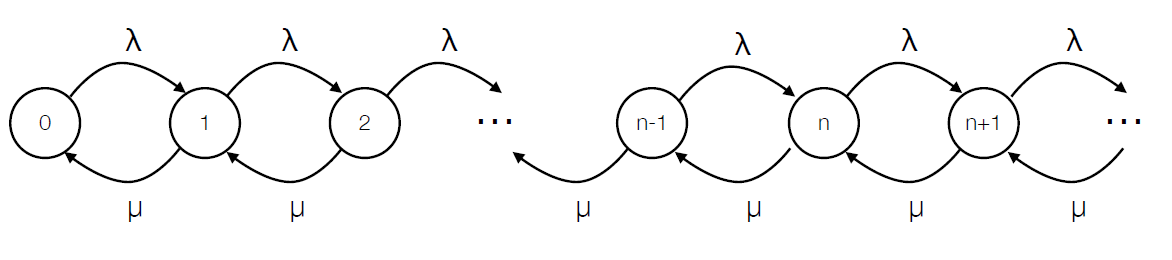
\includegraphics[width=0.3\textwidth]{MM1}
\begin{itemize}
\item Arrival process = $Poisson(\lambda)$
\item Service times = $Exponential(\mu)$
\item Steady state probabilities : 
\\$p_n=(1-\frac{\lambda}{\mu})\left(\frac{\lambda}{\mu}\right)^n=(1-\rho)\rho^n$
\item Average number of clients in system : 
\\$L=\sum_{n=0}^{\infty} np_n=\frac{\lambda}{\mu-\lambda}=\frac{\rho}{1-\rho}$
\item Average time spent in system :
\\$W=L/\lambda=\frac{1}{\mu-\lambda}=\frac{\rho}{\lambda(1-\rho)}$
\item Average time spent in queue :
\\ $W_q=W-\frac{1}{\mu}=\frac{\lambda}{\mu(\mu-\lambda)}=\frac{\rho^2}{\lambda(1-\rho)}$
\item Average number of clients waiting in queue :
\\ $L_q=\lambda W_q=\frac{\lambda^2}{\mu (\mu-\lambda}=\frac{\rho^2}{1-\rho}$
\item $P[W<t|L=n]=\int_0^t \mu \exp^{-\mu \tau}\frac{(\mu\tau)^n}{n!}d\tau$
\item $P[W <t]$
\\$ =\sum_{n=0}^{\infty} P[W <t|L = n]P[L = n]$
\\$=\sum_{n=0}^{\infty} \int_0^t \mu \exp^{-\mu \tau}\frac{(\mu \tau)^n}{n!}d\tau \left( \frac{\lambda}{\mu}\right)^n \left(1-\frac{\lambda}{\mu}\right)$
\\$=\int_0^t (\mu -\lambda) \exp^{-\mu \tau}\sum_{n=0}^{\infty} \frac{(\mu \tau)^n}{n!}d\tau $
\\$=\int_0^t (\mu -\lambda) \exp^{-(\mu-\lambda) \tau}d\tau $
\\$=1-\exp^{(\mu-\lambda)t}$
\end{itemize}

\paragraph{M/M/s queue}~~\\
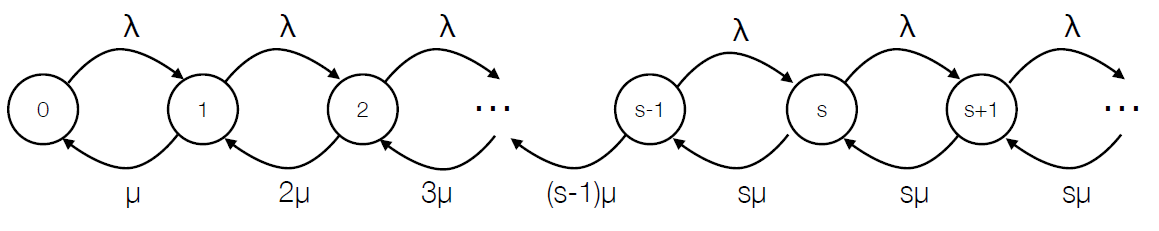
\includegraphics[width=0.3\textwidth]{MMs}
\begin{itemize}
\item Arrival process = $Poisson(\lambda)$
\item Service times = $Exponential(\mu)$ $s$ servers
\item Steady state probabilities : 
\\$p_0=\left(\sum_{n=0}^{s-1} \frac{\lambda^n}{n!\mu^n}+\frac{\lambda^s}{s!\mu^s}\left(\frac{1}{1-\frac{\lambda}{s \mu}}\right) \right)^{-1}$
\\$p_n=\frac{\lambda^n}{n!\mu^n}p_0$ \quad $\forall n\leq s$
\\$p_n=\frac{\lambda^s}{s!\mu^s}\left(\frac{\lambda}{s\mu}\right)^{n-s}p_0$ \quad $\forall n\geq s$
\item Average number of clients waiting in queue :
\\ $L_q=\sum_{n=0}^{\infty}np_{s+n}=p_0\frac{\lambda^*}{s!\mu^s}\frac{\lambda/s\mu}{(1-\lambda/s\mu)^2}$
\item Average time spent in queue : $W_q=L_q/\lambda$
\item Average time spent in system : $W=W_q+\frac{1}{\mu}$
\item Average number of clients in system : 
\\$L=\lambda W=L_q+\frac{\lambda}{\mu}$
\item Taux d'occupation : $\frac{\lambda}{s\mu}$
\end{itemize}
\paragraph{M/M/1/K queue}~~\\
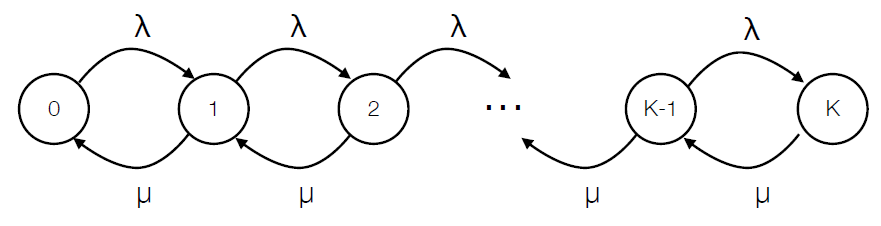
\includegraphics[width=0.3\textwidth]{MMk}
\begin{itemize}
\item Arrival process = $Poisson(\lambda)$
\item Service times = $Exponential(\mu)$ 
\item Maximum number of clients in system = $K$
\item Steady state probabilities : 
\\$p_0=\frac{1-\frac{\lambda}{\mu}}{1-\left(\frac{\lambda}{\mu}\right)^{K+1}}$ \quad si $\lambda\neq \mu$
\\$p_n=\left(\frac{\lambda}{\mu}\right)^np_0$
\item Taux effectif de service: $\lambda(1-p_K)$
\item Quand le taux augmente, le temps d'attente augmente bcp plus pour le même $K$. Il faut donc limiter.
\end{itemize}
\paragraph{M/M/1//N queue}~~\\
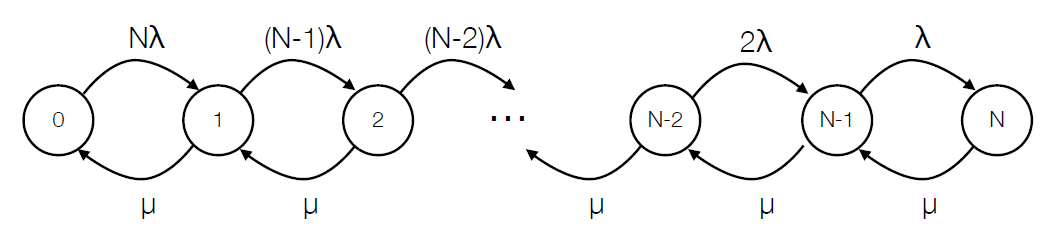
\includegraphics[width=0.3\textwidth]{MMN}
\begin{itemize}
\item Arrival process = $Poisson(\lambda)$ for each potential client
\item Service times = $Exponential(\mu)$ 
\item Steady state probabilities : 
\\$p_n=\frac{N!}{(N-n)!}\left(\frac{\lambda}{\mu}\right)^n p_0$
\end{itemize}
\paragraph{Réversibilité}
\begin{itemize}
\item Le processus inverse est aussi un processus de Markov avec des temps de $\sim expo(\nu_i)$ et des probabilités de transition $p_{ij}^*$
\item Un processus sera dit réversible si $q_{ij}^*= q_{ij}$
\item \textbf{Lemme 1} Soit un processus de Markov pour lequel les probabilités stationnaires existent avec $\sum_ip_i\nu_i<\infty $ alors le processus est réversible $\Leftrightarrow$ la chaîne sous-jacente est réversible.
\item \textbf{Théorème 2} Pour un processus de Markov irréductible, soit des valeurs $\{p_i > 0\}$ avec
\\$\sum_i p_i=1$ \quad $\sum_i p_i \nu_i<\infty$ \quad $p_i q_{ij}=p_jq_{ij}$ $\forall ij$.
\\Alors les $\{p_i\}$ sont les probabilités stationnaires du processus et celui-ci est réversible avec une chaîne sous-jacente récurrente-positive.
\item \textbf{Théorème 3} Pour un processus de Markov irréductible, supposons que nous ayons des valeurs $\{p_i > 0\}$ et $\{q_{ij}^*\geq 0\}$ telles que 
$\sum_i p_i=1$ \quad $\sum_i p_i \nu_i<\infty$ \quad $\sum_j q_{ij}=\sum_j q_{ij}^*$ \quad $p_iq_{ij}=p_jq_{ji}^*$ $\forall ij$.
\\Alors les $\{p_i \}$ sont les probabilités stationnaires du processus et celui-ci est récurrent positif et $\{q_{ij}^* \}$ sont les taux de transition du processus inverse.
\item \textbf{Théorème 4} Les processus de naissance et de mort sont réversibles s’il existe des $p_i > 0$ tels que
$\sum_i p_i=1$ \quad $\sum_i p_i \nu_i<\infty$ \quad $p_i \lambda_i=p_{i+1}\mu_{i+1}$.
\item \textbf{Théorème de Burke}
\begin{enumerate}
\item Le processus de départ d’un système M/M/1 est un processus de Poisson
\item L’état du système au temps $t$ est indépendant des départs avant $t$.
\item En cas de service FCFS, le temps de séjour d’un client qui quitte le système en $t$ est indépendant des départs avant $t$.
\end{enumerate}
\end{itemize}
\paragraph{Systèmes de files d’attente en série}
\begin{enumerate}
\item Si les arrivées suivent un processus de Poisson et que les temps de services sont distribués exponentiellement pour chaque serveur (avec éventuellement des taux de service différents), les deux systèmes se comporteront comme des systèmes M/M/1.
\item Les états des deux systèmes à un moment $t$ sont indépendants
\item Le temps de séjour d’un client est indépendant dans chaque file.
\end{enumerate}
\paragraph{Système de file d’attente avec retour}
\begin{enumerate}
\item Les arrivées externes suivent un processus de Poisson.
\item Les arrivées dans la file ne forment pas un processus de Poisson (somme de deux processus de poisson qui ne sont pas indépendants)
\item Le système global se comporte comme un système
M/M/1 (un retour n’implique pas de changement d’état).
\end{enumerate}
\paragraph{Réseaux de files d’attentes}
\begin{enumerate}
\item Soit un réseau de files d’attentes (stations) avec des arrivées externes suivant des processus de Poisson, 
\item il y a $K$ stations avec une file et un ou plusieurs serveurs, 
\item un job qui quitte une station est envoyé vers d’autres stations (ou quitte le système) avec des probabilités qui ne dépendent pas de son parcours antérieur (une autre manière de voir est que tous les jobs qui quittent une station sont considérés identiques et indépendants).
\item On peut montrer que le processus de Markov qui
représente le système est réversible.
\item Si toutes les stations ont un seul serveur, alors la probabilité stationnaire d’avoir $m_i$ jobs présents à la station $i$ ($\forall i$) est $\prod_{i=1}^K \rho_i^{m_i}(1-\rho_i)$
\item Pour un moment donné t, le nombre de jobs présents à chaque station est indépendant du nombre de jobs présents aux autres stations. Les processus ne sont cependant pas indépendants.
\item Les flux sortants forment des processus de Poisson, par contre les flux entre les stations ne forment pas des processus de Poisson.
\end{enumerate}
\section{Fluid Approximation for non-stationary queueing systems}
\paragraph{Transient behavior}~~\\
When a queue operates in steady state, queues are produced by random variability
\\A nonstationary arrival pattern presents an additional source of variability : predictable variability
\begin{itemize}
\item Relaxation time: time it takes for the system to forget  and to reach the steady state 
\\$\Rightarrow$ approx: $T_0=\frac{\lambda/s\mu+C^2(s)}{(1-\lambda/s\mu)^2}\frac{1}{ s\mu}$
\end{itemize}
If the arrival and service processes stay the same during a period of length $T_0$, then it can be assumed that the probability of the system being in any state is the steady state probability.
\paragraph{Non-stationnary Poisson process}
~~\\
Independant increments
\begin{itemize}
\item $\lambda(t)$= the arrival rate at time $t$
\item Expected number of arrivals until time $t$ is $\int_0^t \lambda(\tau)d\tau$.
\item Expected number arrivals between $a$ and $b$ is equal to $\int_a^b \lambda(\tau)d\tau=\Lambda(b)-\Lambda(a)$.
\item $P[n$ arrivals between $a$ and $b$]\\ $=\dfrac{(\Lambda(b)-\Lambda(a))^n \exp^{-(\Lambda(b)-\Lambda(a))}}{n!}$
\item Distribution of unordered arrivals:
\\$P[$one of the arrivals before $t|N(t)]$ =$\frac{\Lambda(t)}{\Lambda(T)}$
\item Ordered arrivals : 
\\$P[$first arrival before $t|N(T) = n]$\\ 
$= 1- P[$all arrivals after $ t|N(T) = n]$
\\$= 1-\left(\frac{\Lambda(T)-\lambda(t)}{\Lambda(T)}\right)^n$
\end{itemize}
\paragraph{Nonstationnary queuing systems}
\begin{itemize}
\item Arrival rate varies slowly and load stays below $1$ $\Rightarrow$ quasi-steady state approximation
\item Load goes higher than $1$ $\Rightarrow$ fluid approximation
\item Arrival rate varies quickly and load stays below $1$ $\Rightarrow$ most difficult situation, as an approximation use steady state results on average load
\end{itemize}
\paragraph{Quasi Steady-state approximation}~~\\
Validity of approximation if
\begin{itemize}
\item one server system (M/M/1 or M/G/1):
\\$\Delta=\left|\frac{d\rho(t)}{dt}\right|\frac{1}{\mu(t)} \frac{1}{(1-\rho(t))^3)}<<1$
\item  multiple server system: $\Delta=\left|\frac{d\bar{\rho}(t)}{dt}\right|\frac{1}{s(t)\mu(t)} \frac{1}{(1-\bar{\rho}(t))^3)}<<1$ with $\bar{\rho}(t)=\lambda(t)/s(t)\mu(t)$
\end{itemize}
\paragraph{Fluid approximation}~~\\
For short service times and large loads
\begin{itemize}
\item the predictable variability will be much larger than the random variability
\item we can use a deterministic model
\item the principle of this approximation is analogous to models of fluids
\end{itemize}
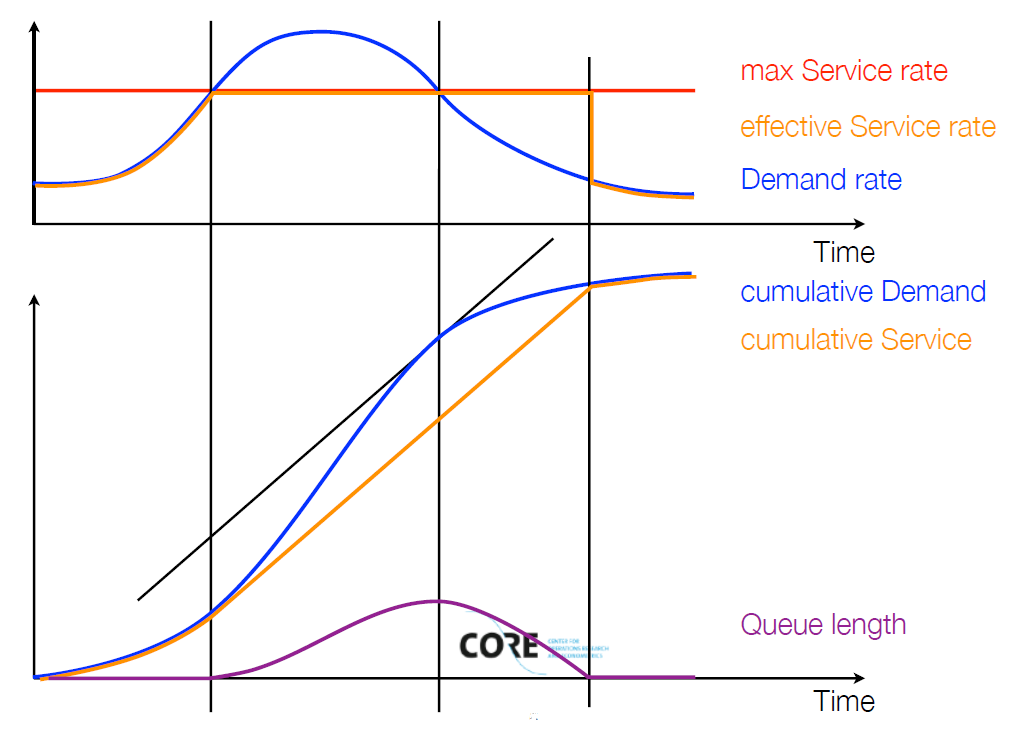
\includegraphics[width=0.3\textwidth]{fluid}
Notation
\begin{itemize}
\item $c =$ combined service rate among all servers (constant in this part)
\item $\lambda(t) =$ arrival rate at time $t$ (we neglect variability)
\item $A(t) =\int_0^t \lambda(\tau) d\tau$ cumulative number of arrivals up to time $t$
\item $\omega(t) =$ departure rate from the queue at time $t$ (we neglect variability)
\item $D_q(t)=\int_0^t \omega(\tau)d\tau$ cumulative number of departures from the queue up to time $t$
\item $ L_q(t) = A(t) - D_q(t)$ number of customers waiting at time $t$.
\end{itemize}
Approximation
\begin{itemize}
\item No queue regime: If $L_q(t) = 0$ and $\lambda(t) < c$ \\ then $\frac{dL_q(t)}{dt} = 0$ and $\omega(t)=\lambda(t)$
\item Queue growth regime: If $\lambda(t)\geq c$ \\ then $\frac{dL_q(t)}{dt} = \lambda(t)-c\geq  0$ and $\omega(t) = c$
\item Queue decline regime: If $L_q(t) > 0$ and $\lambda(t) < c$ \\ then 
$\frac{dL_q(t)}{dt} = \lambda(t) - c < 0$ and $\omega(t) = c$
\end{itemize}
\paragraph{Limits of fluid approximation}
\begin{itemize}
\item Long service times
\item Ignores variability
\begin{itemize}
\item when $\rho(t) << 1$ use quasi-steady state model
\item when $\rho(t) \leq  1$ and $1-\rho(t)<<1$ 1 approximation is difficult
\begin{itemize}
\item diffusion approximations
\item if the process stays during a long time in this zone then chose $\bar{\rho}$ and use steady state results
\item if the process does not stay in this zone then ignore the problem
\end{itemize}
\item when $\rho(t) > 1$ the fluid approximation will correctly estimate queue growth
\end{itemize}
\end{itemize}
\paragraph{Queueing to meet a schedule}~~\\
In many situations, nonstationary arrival rates come from the fact that customers want to depart from the service system according to a schedule
\begin{itemize}
\item If the system capacity is larger than the desired arrival rate, then there will be no queue
\item If the system capacity is smaller than the desired arrival rate, then some customers will have to arrive earlier than desired (or later)
\end{itemize}
\paragraph{Optimal capacity}~~\\
\begin{itemize}
\item A relatively small increase in service capacity can have a large impact on waiting time
\item Suppose we face a nonstationary arrival process and we want to find the optimal (constant) service capacity in order to minimize the service cost and the waiting cost of customers: $\min C_s + C_w$
\begin{itemize}
\item service cost per period $= C_s =\alpha c$
\begin{itemize}
\item $\alpha =$ service cost per unit of capacity for one period
\item $c=$ capacity (customers/unit of time)
\end{itemize}
\item waiting cost per period $= C_w =\beta W(c)$
\begin{itemize}
\item $\beta =$ value of customer time
\item $W(c) =$ total waiting time per period
\end{itemize}
\end{itemize}
\item Solution through marginal analysis
\\ $\Delta C = \alpha \Delta c + \beta [W(c+\Delta c) -W(c)]$
\\$\Rightarrow W(c)-W(c+\Delta c)=\frac{T(c)^2 \Delta c}{2}$
\\$\Rightarrow \Delta C=\alpha \Delta c-\beta \frac{T(c)^2 \Delta c}{2}=\Delta c \left(\alpha -\beta \frac{T(c)^2}{2}\right)$
\\Optimaliy $\Rightarrow T^*(c)=\sqrt{\frac{2\alpha}{\beta}} $ 
\end{itemize}
\paragraph{Varying service capacity} ~~\\
Suppose the facility operates at a fixed capacity, but in order to cope with a nonstationary arrival rate, the capacity is increased by a fixed amount during a certain period
\begin{itemize}
\item when do we schedule this extra capacity: as early as possible while still being able to use the full additional capacity
\item for how long do we schedule this extra capacity: $Area=[(c_2-c_1)\Delta t]t_2$
\item if a break must be scheduled, when do we schedule it: If the break cannot be scheduled during the low-arrival period, it should be scheduled as late as possible.
\end{itemize}
Notation
\begin{itemize}
\item $\gamma=$ cost of supplementing capacity, per unit time
\item $\beta=$value of customer time
\item $c_1 =$ normal service capacity
\item $c_2=$ capacity during period of increased capacity
\end{itemize}
\paragraph{Scheduling for a varying capacity}~~\\
Once a capacity profile has been determined (through quasi-steady state or fluid models), we must decide how to schedule workers to attain this capacity.
\\ Mathematical programming:
$\min \sum_i c_i x_i$
\\$\sum_i a_{ij}x_i\geq r_j$ $\forall j$
\\$x_i \in \mathbb{N}$
\\where
\begin{itemize}
\item $x_i =$ number of workers on schedule $i$
\item $a_{ij}=\begin{cases} 1 & \text{if schedule $i$ includes period $j$}\\0 & \text{otherwise} \end{cases}$
\item $r_j = $ number of workers needed for period j
\end{itemize}



\section{Tools}
\begin{itemize}
\item $\sum_{k=1}^n k^2=\frac{n(n+1)(2n+1)}{6}$
\item $\sum_{k=0}^n=\frac{1-a^{n+1}}{1-a}$
\end{itemize}








\end{multicols}

\begin{table}[H]
    \centering
    \begin{tabu} to \textwidth{@{}|ll|cccc|@{}}
    \toprule
    Nom& & Domaine & Densité & Espérance & Variance\\
     \midrule
    Exponentielle & Expo($\lambda$)& $x\in \mathbb{R}_+$ & $\lambda exp(-\lambda x)$& $\frac{1}{x}$ & $\frac{1}{\lambda^2}$\\
        Erlang & Erlang($\lambda,n$)& $x\in  \mathbb{R}_+$ & $\frac{\lambda^n x^{x-1}}{(n-1)!}\exp{(-\lambda x)}$ & $\frac{n}{\lambda}$& $\frac{n}{\lambda^2}$\\
        Gaussienne & $\mathcal{N}(\mu, \sigma)$& $x\in \mathbb{R}$& $\frac{1}{\sigma\sqrt{2\pi}}\exp{\left( \frac{-(x-\mu)^2}{2\sigma^2}\right)}$& $\mu$ & $\sigma$\\
        Uniforme & $U(a,b)$ & $x \in [a,b]$& $\frac{1}{b-a}$ & $\frac{a+b}{2}$ & $\frac{(b-a)^2}{12}$\\
        Bernoulli & $B(p)$ & $\{0,1\}$ & $P(0)=1-p,P(1)=p$& $p$ & $p(1-p)$\\
        Binomiale & $Bin(p,n)$ & $0\leq k \leq n$& $\frac{n!}{k!(n-k)!}p^k(1-p)^{n-k}$& $np$& $np(1-p)$\\
        Géométrique & $Geo(p)$ & $n\in \mathbb{N}$ & $p^n(1-p)$& $\frac{p}{1-p}$ & $\frac{p}{(1-p)^2}$\\
        Poisson & $Po(\lambda)$ & $n\in \mathbb{N}$ & $\frac{\lambda^n}{n!}\exp{(-\lambda)}$ & $\lambda$ & $\lambda$\\       
        \bottomrule
    \end{tabu}
\end{table}



\end{document}
